\part{Basic computer architecture}
\frame{\partpage}

\begin{frame}{What is a computer?}
	\begin{itemize}
		\item In \textbf{groups of 2-3}
		\item Discuss for \textbf{10 minutes}
		\item Go to \url{www.socrative.com} (or open the Socrative app) and enter room code \texttt{FALCOMPED}
		\item \textbf{Individually}, suggest a \textbf{one sentence} definition for a computer
	\end{itemize}
\end{frame}

\begin{frame}{The Von Neumann model}
	\begin{center}
		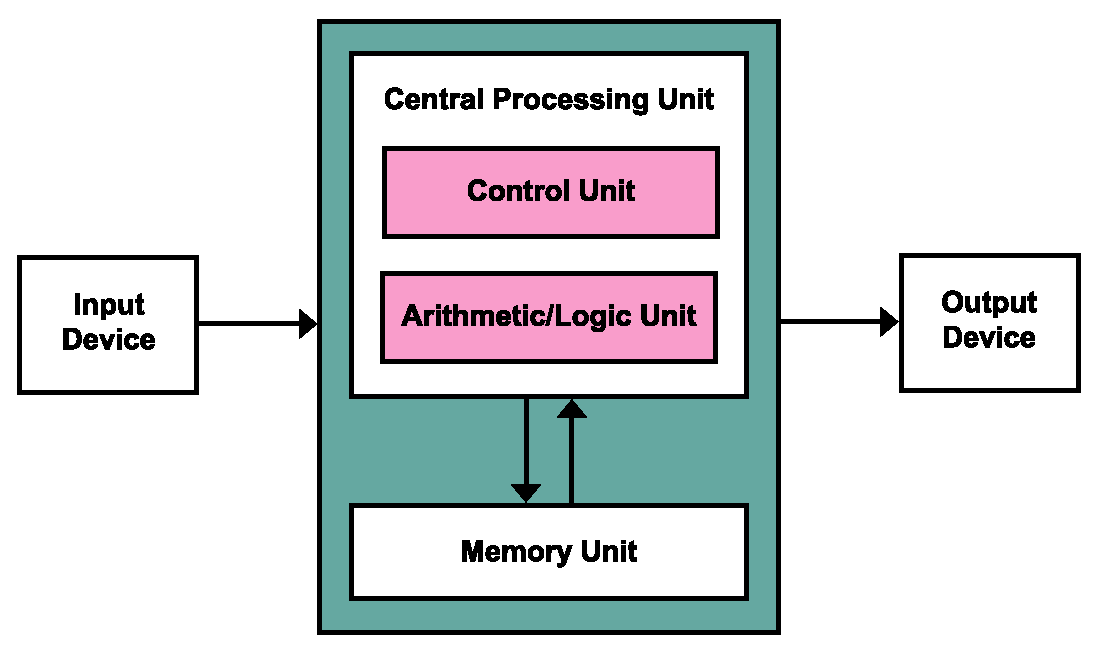
\includegraphics[height=0.7\textheight]{vonneumann}
	\end{center}
\end{frame}

\begin{frame}{Modern PC architecture}
	\begin{center}
		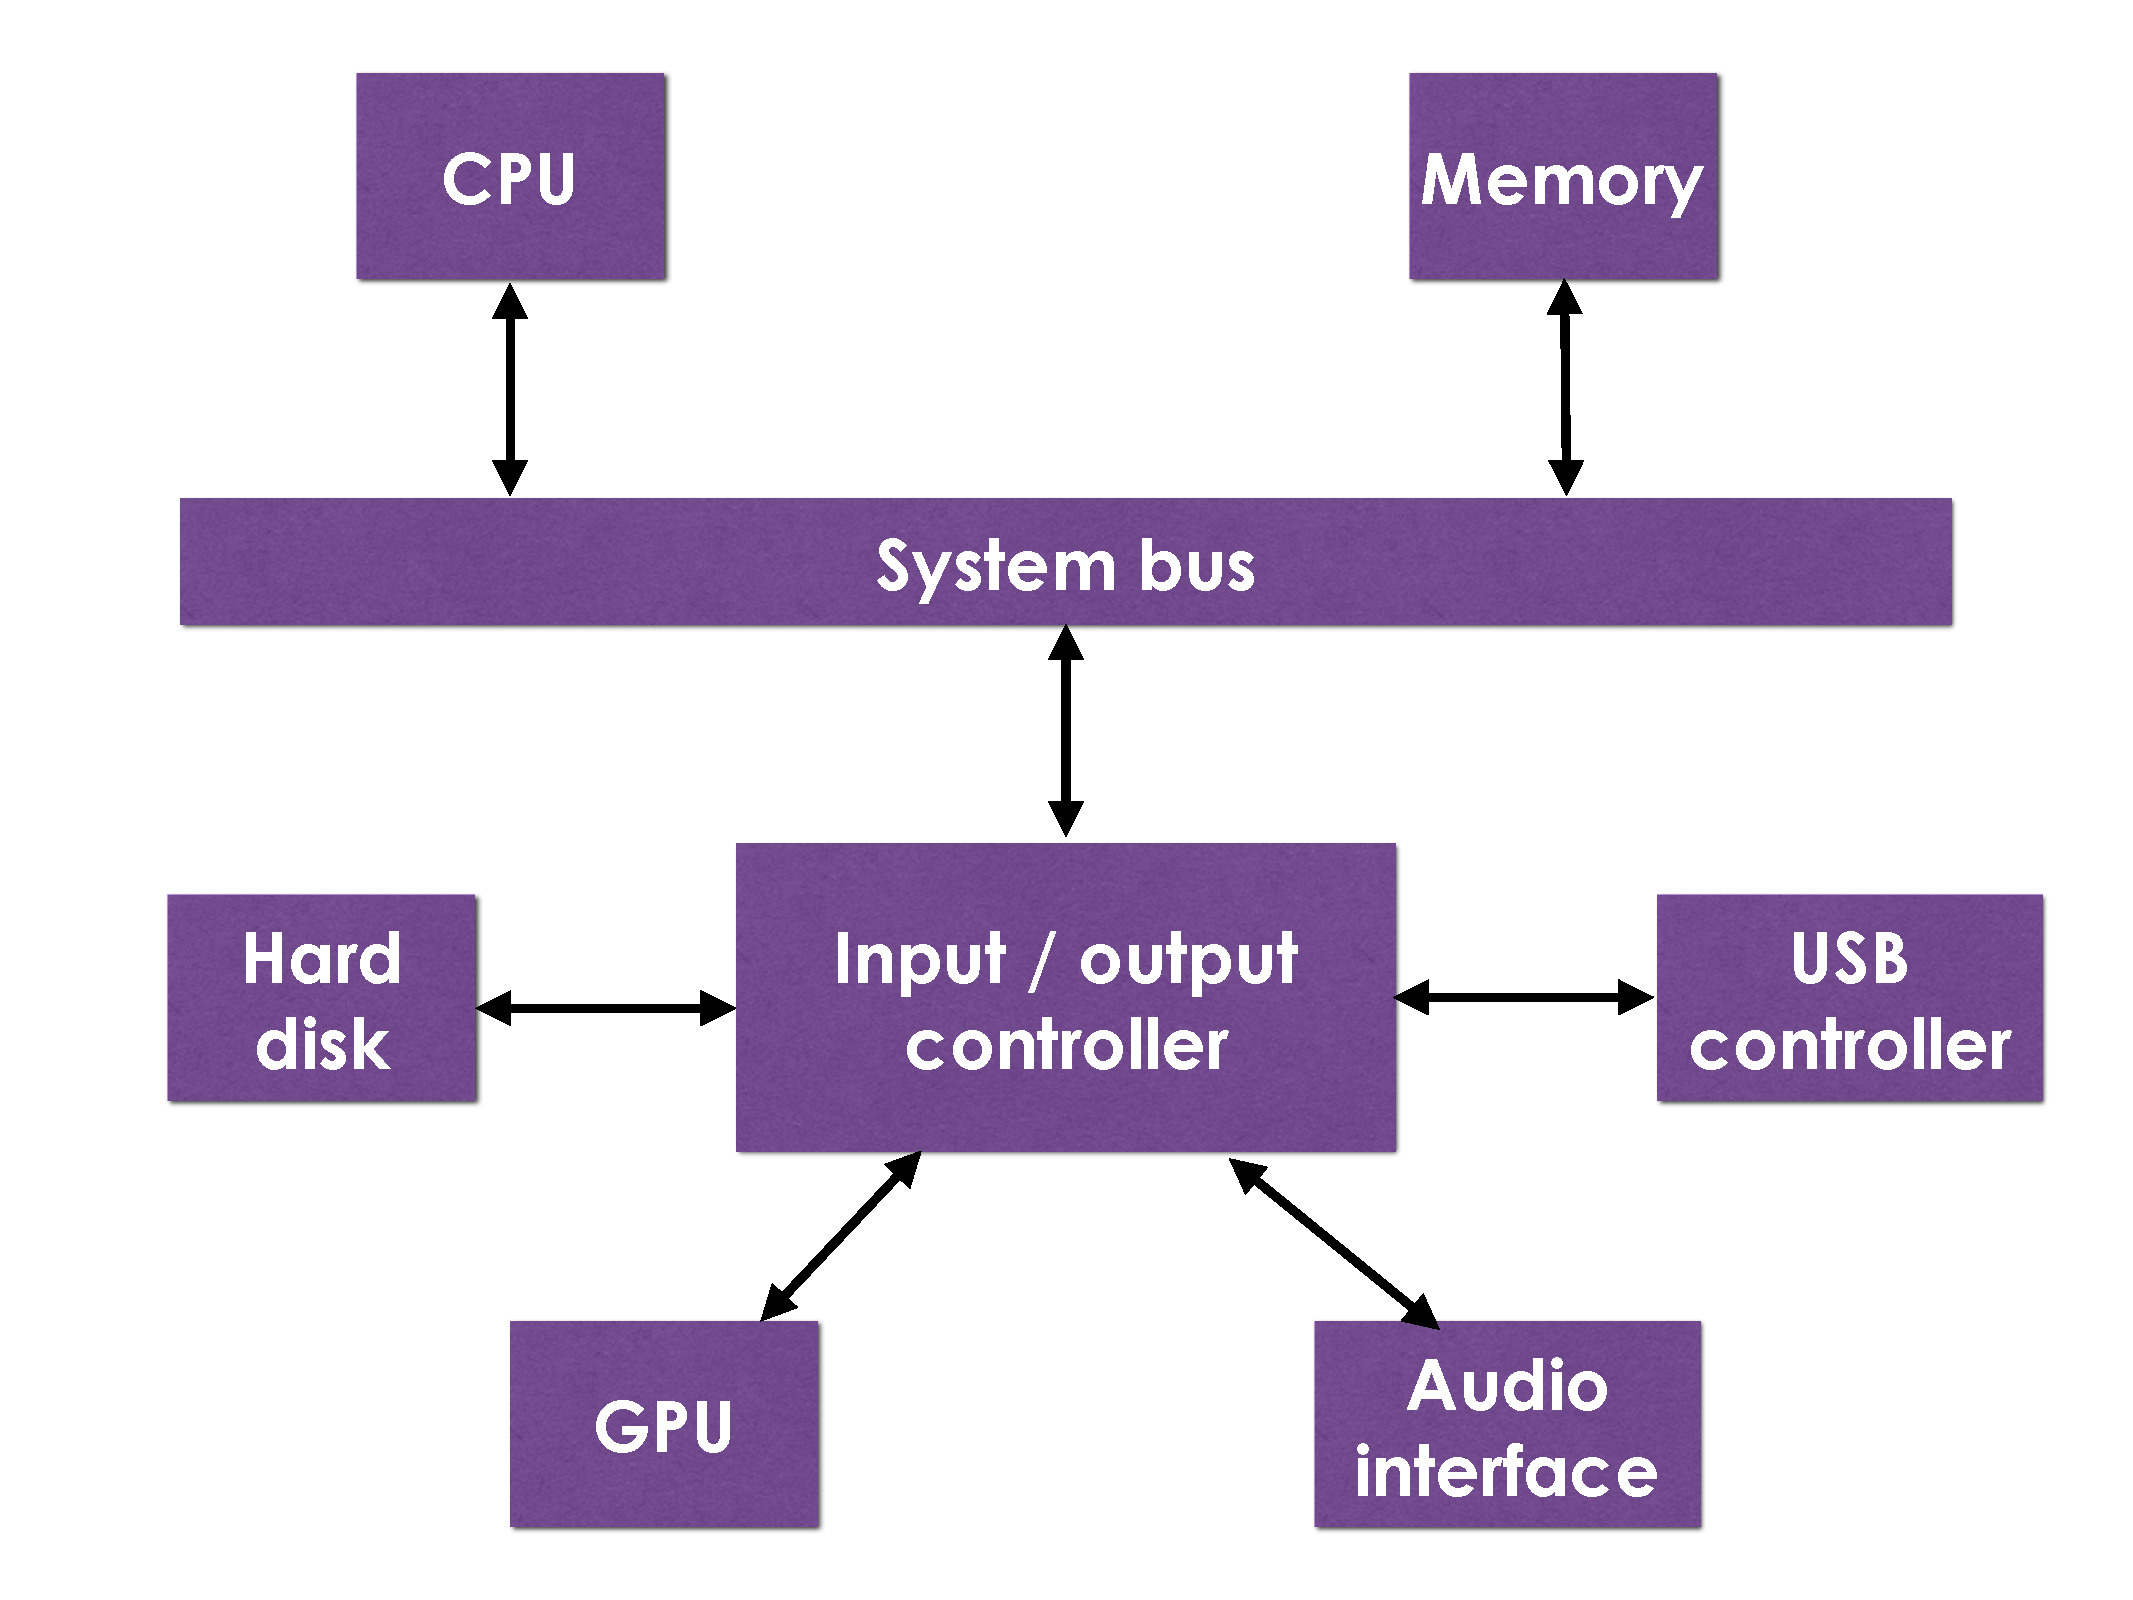
\includegraphics[height=0.7\textheight]{architecture-diagram}
	\end{center}
\end{frame}

\begin{frame}{Central processing unit (CPU)}
	\pause Carries out
	\begin{itemize}
		\pause \item Arithmetic operations
		\pause \item Logic operations
		\pause \item Control operations
	\end{itemize}
\end{frame}

\begin{frame}{Storage}
	\begin{itemize}
		\pause \item Primary storage
			\begin{itemize}
				\pause \item Directly accessible by the CPU
				\pause \item Random access memory (RAM)
				\pause \item Volatile --- loses its contents when switched off
			\end{itemize}
		\pause \item Secondary storage
			\begin{itemize}
				\pause \item E.g.\ hard disk, SSD, USB flash drive, DVD
				\pause \item Non-volatile --- keeps its contents when switched off
			\end{itemize}
	\end{itemize}
\end{frame}

\begin{frame}{Graphics processing unit (GPU)}
	\begin{itemize}
		\pause \item Responsible for displaying images on screen
		\pause \item Traditionally, one of many input/output devices
		\pause \item Nowadays, essentially a highly specialised CPU with its own primary storage
	\end{itemize}
\end{frame}

\begin{frame}{The stored program architecture}
	\begin{itemize}
		\pause \item A \textbf{computer program} is a sequence of instructions for the CPU
			\begin{itemize}
				\pause \item (Note: it's spelled ``program'', not ``programme'')
			\end{itemize}
		\pause \item The \textbf{programmable computer} --- can carry out different tasks depending on what program it is given
		\pause \item Most modern computers use the \textbf{same} memory to store the program and the data it uses
	\end{itemize}
\end{frame}

